\chapter{Implementación del software\label{sec:Implementacion_soft}}

Una vez finalizado el soporte físico del sistema, será necesario implementar a nivel de software todas las funciones deseadas.

El sistema está compuesto por tres microcontroladores, cada uno de ellos con sus propias características y métodos de programación. Debido a esto, a lo largo de este capítulo se explicará con detenimiento el software utilizado individualmente para ellos así como los distintos entornos de desarrollo (\acrshort{IDE}) necesarios.

Los distintos elementos se presentarán siguiendo el mismo orden que la información que se desea adquirir. Este es:
ADS $\Rightarrow$ Microcontrolador $\Rightarrow$ Interfaz inalámbrica $\Rightarrow$ PC.

\section{Microcontrolador STM32F4\label{Software_micro}}

Debido a la complejidad de los microcontroladores de la familia STM32, los desarrolladores han dedicado su tiempo y esfuerzo en crear herramientas que faciliten su programación. Estas herramientas llamadas \acrshort{IDE} contienen una recopilación de funciones, utilidades y ejemplos que simplifican sensiblemente el proceso de diseño e implementación del software que ejecutará el microcontrolador.

Es tan grande la comunidad de desarrolladores que hay detrás del STM que numerosas empresas han visto como una oportunidad de negocio la creación de un \acrshort{IDE} propietario.

\clearpage

\begin{figure} [h]
    \centering
    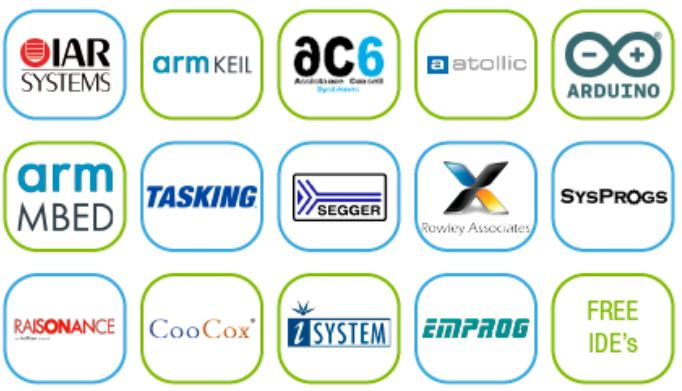
\includegraphics[width=13cm]{STM32_IDEs}
    \caption{IDE's alternativos disponibles \cite{STM32_IDEs}}
    \label{fig:STM32_IDEs}
\end{figure}

La figura \ref{fig:STM32_IDEs} muestra algunos entornos de desarrollo recomendados por el fabricante en su propia página web. Como se puede apreciar, en la imagen se hace distinción entre las opciones comerciales (azul) y las gratuitas (verde).

Uno de los objetivos de este proyecto era utilizar Software Libre en la medida de lo posible. Por ese motivo se probaron algunas de las alternativas presentes en la imagen anterior así como otras menos conocidas basadas en Oracle como "System Workbench for STM32". A continuación se presentan algunas de las utilizadas al comienzo del proyecto junto con sus características y el motivo de su descarte:
\begin{itemize}
   \item \textbf{CooCox}: Presenta muchos ejemplos prácticos pero su interfaz es muy lenta. Necesita demasiado tiempo para iniciar.
   \item \textbf{Arduino}: Fase muy temprana de desarrollo.
   \item \textbf{System Workbench for STM32} Buena comunidad respaldando pero incompatible con las herramientas de STM.

\begin{figure} [h]
    \centering
    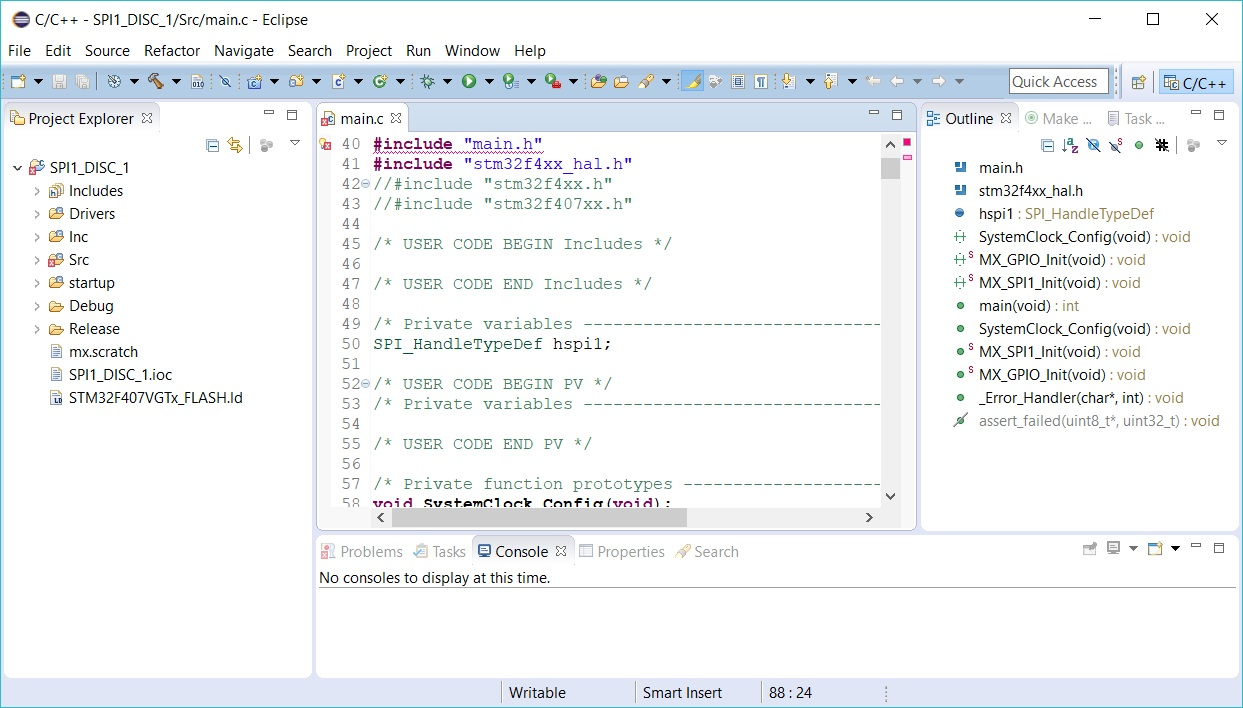
\includegraphics[width=13cm]{Alternative_IDE}
    \caption{Ejemplo de \acrshort{IDE} alternativo}
    \label{fig:Alternative_IDE}
\end{figure}

Finalmente se optó por armKeil, pues tiene una gran cantidad de ejemplos y librerías descargables desde la propia interfaz, contiene un gran número de funciones adicionales y la compatibilidad con las herramientas de STM es muy buena. Aunque en la figura \ref{fig:STM32_IDEs} aparece entre las alternativas gratuitas se debe destacar que cuenta con dos versiones, una gratuita que permite realizar proyectos básicos y otra comercial destinada a aplicaciones de mayor envergadura. La limitación impuesta en la versión gratuita consiste en una limitación en la cantidad de código que la herramienta permite compilar.



Software
	Comunicación ADS - STM
	
	Comunicación STM- ESP
	
	Arduino (Comunicación ESP - PC)
	
	
